\renewcommand*{\arraystretch}{1.1}

\subsection*{BI / read / 3}
\label{section:bi-read-03}

\renewcommand{\currentQueryCard}{3}
    \marginpar{
	\raggedleft
	\vspace{0.22ex}

    \queryRefCard{bi-read-01}{BI}{1}\\
    \queryRefCard{bi-read-02}{BI}{2}\\
    \queryRefCard{bi-read-03}{BI}{3}\\
    \queryRefCard{bi-read-04}{BI}{4}\\
    \queryRefCard{bi-read-05}{BI}{5}\\
    \queryRefCard{bi-read-06}{BI}{6}\\
    \queryRefCard{bi-read-07}{BI}{7}\\
    \queryRefCard{bi-read-08}{BI}{8}\\
    \queryRefCard{bi-read-09}{BI}{9}\\
    \queryRefCard{bi-read-10}{BI}{10}\\
    \queryRefCard{bi-read-11}{BI}{11}\\
    \queryRefCard{bi-read-12}{BI}{12}\\
    \queryRefCard{bi-read-13}{BI}{13}\\
    \queryRefCard{bi-read-14}{BI}{14}\\
    \queryRefCard{bi-read-15}{BI}{15}\\
    \queryRefCard{bi-read-16}{BI}{16}\\
    \queryRefCard{bi-read-17}{BI}{17}\\
    \queryRefCard{bi-read-18}{BI}{18}\\
    \queryRefCard{bi-read-19}{BI}{19}\\
    \queryRefCard{bi-read-20}{BI}{20}\\
    \queryRefCard{bi-read-21}{BI}{21}\\
    \queryRefCard{bi-read-22}{BI}{22}\\
    \queryRefCard{bi-read-23}{BI}{23}\\
    \queryRefCard{bi-read-24}{BI}{24}\\
    \queryRefCard{bi-read-25}{BI}{25}\\
}



\noindent\begin{tabularx}{\queryCardWidth}{|>{\queryPropertyCell}p{\queryPropertyCellWidth}|X|}
	\hline
	query & BI / read / 3 \\ \hline
%
	title & Tag evolution
 \\ \hline
%
	pattern & \hfill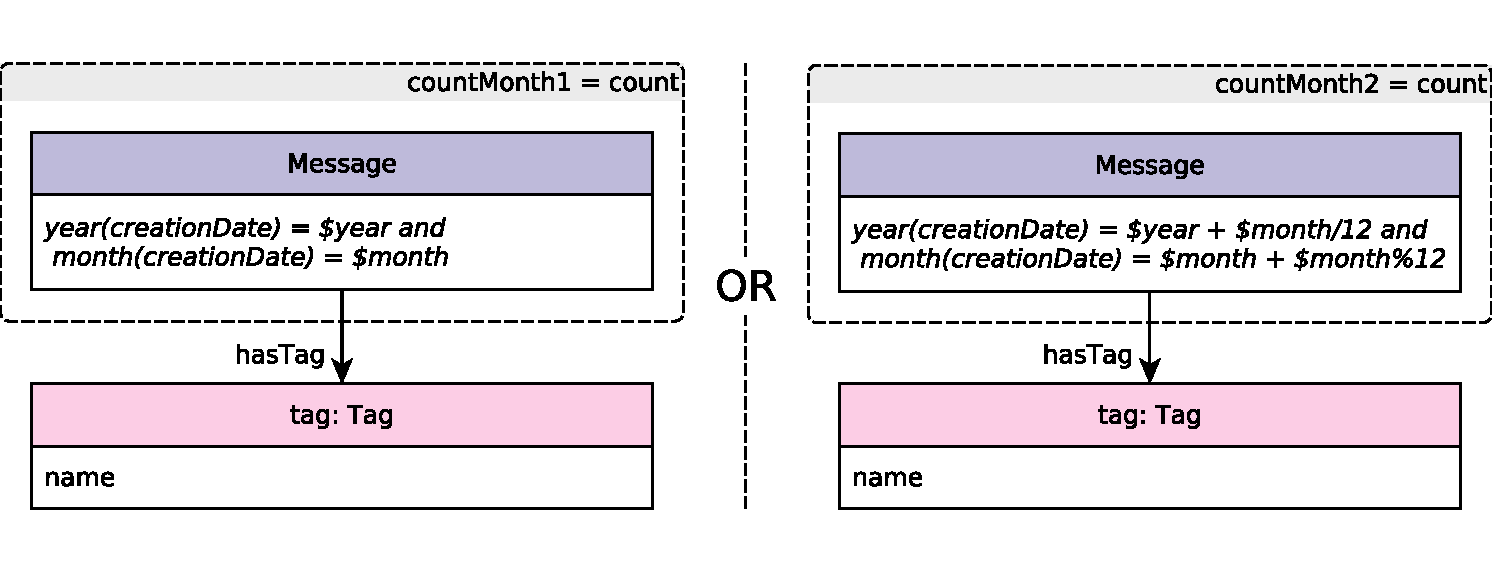
\includegraphics[scale=\patternscale,margin=0cm .2cm]{patterns/bi-read-03}\hfill\vadjust{} \\ \hline
%
	desc. & Find the \emph{Tags} that were used in \emph{Messages} during the given
\texttt{month} of the given \texttt{year} and the \emph{Tags} that were
used during the next month.

For both months, compute the count of \emph{Messages} that used each of
the \emph{Tags}.
 \\ \hline
%
	
		params &
		\innerCardVSpace{\begin{tabularx}{\attributeCardWidth}{|>{\paramNumberCell}c|>{\varNameCell}M|>{\typeCell}m{\typeWidth}|Y|} \hline
		$\mathsf{1}$ & year
 & 32-bit Integer
 &  \\ \hline
		$\mathsf{2}$ & month
 & 32-bit Integer
 &  \\ \hline
		\end{tabularx}}\innerCardVSpace \\ \hline
	
%
	
		result &
		\innerCardVSpace{\begin{tabularx}{\attributeCardWidth}{|>{\resultNumberCell}c|>{\varNameCell}M|>{\typeCell}m{\typeWidth}|>{\resultOriginCell}c|Y|} \hline
		$\mathsf{1}$ & tag.name & String & R &
				 \\ \hline
		$\mathsf{2}$ & countMonth1 & 32-bit Integer & A &
				Occurrences of the tag during the given \texttt{year} and \texttt{month}
 \\ \hline
		$\mathsf{3}$ & countMonth2 & 32-bit Integer & A &
				Occurrences of the tag during the next month after the given
\texttt{year} and \texttt{month}
 \\ \hline
		$\mathsf{4}$ & diff & 32-bit Integer & A &
				Absolute difference of \texttt{countMonth1} and \texttt{countMonth2}
 \\ \hline
		\end{tabularx}}\innerCardVSpace \\ \hline
	
%
	
		sort		&
		\innerCardVSpace{\begin{tabularx}{\attributeCardWidth}{|>{\sortNumberCell}c|>{\varNameCell}M|>{\directionCell}c|Y|} \hline
		$\mathsf{1}$ & diff
 & $\desc
$ &  \\ \hline
		$\mathsf{2}$ & tag.name
 & $\asc
$ &  \\ \hline
		\end{tabularx}}\innerCardVSpace \\ \hline
	%
	limit & 100 \\ \hline
	%
	CPs &
	\multicolumn{1}{>{\raggedright}l|}{
		\chokePoint{2.4}, 
		\chokePoint{3.1}, 
		\chokePoint{3.2}, 
		\chokePoint{4.1}, 
		\chokePoint{4.3}, 
		\chokePoint{5.3}, 
		\chokePoint{6.1}
		} \\ \hline
	%
	%
\end{tabularx}
\queryCardVSpace